\chapter{实验与分析}

本章从实验的角度验证系统的有效性，分别对时空预测模型的预测性能、智能体在真实交通场景中的意图识别与工具调度能力、系统整体架构的鲁棒性以及各模块的实际贡献进行评估。

\section{实验准备与环境设置}

\subsection{实验数据集与数据预处理}

本文使用 PeMS08（Caltrans Performance Measurement System）数据集进行实验。PeMS08 是加州交通局发布的真实高速公路交通数据集，采集自洛杉矶县区高速公路的传感器网络。该数据集包含了 2016 年 7 月至 8 月间 170 个传感器节点的交通数据，采样间隔为 5 分钟一次，每个采样点记录了车流量、平均车速和道路占有率三个指标。传感器覆盖了多条主要高速公路的路段，节点之间的空间分布反映了实际路网的拓扑结构。数据集的总体时间跨度为两个月，涵盖了完整的日周期和周周期变化规律，包括工作日早晚高峰和周末的低流量时段等典型的交通模式。

原始数据以 csv 格式保存，每个传感器的数据存储在独立的文件中。由于不同传感器的数据采集时间不完全同步，加上通信故障和设备维护等因素，原始数据中存在缺失值、异常值和重复记录。在进行模型训练和智能体推理之前，需要对这些原始数据进行统一的预处理。整个预处理流程分为四个步骤。

第一步是数据清洗。缺失值的情况比较常见，比如某个传感器在某个时间段内因为临时故障没有上报数据。对于持续时间在 3 个时间步以内的短时缺失，采用相邻时间窗口的均值进行插补，具体做法是用缺失点前后各 2 个时间步的观测值取平均填入。对于持续时间超过 6 个时间步（30 分钟）的连续缺失，直接标记为无效，不进行插补，以避免引入过多的人工噪声影响模型训练。异常值的检测则基于 3-sigma 原则，计算每个传感器的流量、速度和占有率三个指标的均值和标准差，如果某个观测值与均值的偏差超过 3 倍标准差，就认为它是一个异常值，用相邻正常值的均值替换。此外，对于速度超过道路限速上限的极值（比如高速公路路段出现 200 km/h 以上的记录）和流量为负的明显错误数据，也一并作为异常值处理。

第二步是时间对齐。不同传感器之间的数据虽然都是以 5 分钟为间隔采集的，但由于各个传感器的时钟存在微小偏差和通信延迟的影响，实际记录的时间戳并不完全对齐在整点间隔上。有的传感器记录的时间可能是 08:00:12，有的是 07:59:48。如果不对齐就直接做时空建模，模型会误以为这些数据来自不同的时间点。具体做法是先确定整个数据集的时间范围（2016 年 7 月 1 日 00:00:00 至 2016 年 8 月 31 日 23:55:00），然后以 5 分钟为步长生成统一的时间网格，共 17856 个时间步。再将每个传感器的数据映射到这个时间网格上，每个时间步取该 5 分钟区间内出现的记录的平均值。如果某个传感器在某个时间步上没有记录，在对应的位置上填入 0。经过对齐之后，所有 170 个传感器都拥有完全相同的 17856 个时间步，形成一个尺寸为 17856 × 170 × 3 的完整时空张量。

第三步是数据标准化。交通流量的数值范围在不同传感器之间差异很大——某些路段由于位于城市主干道，车流量可能达到上千辆每小时，而另一些支线路段可能只有几十辆每小时。如果直接用原始数值进行训练，模型会倾向于关注数值较大的特征而忽略数值较小的特征，影响训练效果。为了消除这种量纲差异，对所有的流量、速度和占有率数据分别做 Z-score 标准化，使每个特征的均值为 0、方差为 1。标准化的均值和方差从训练集中计算得到，然后应用到验证集和测试集上。这样做的原因是保证测试数据在标准化时使用的是训练集的统计量，而不是测试集本身的统计量，避免测试数据的信息泄露到训练过程中。

第四步是原子文件格式化。经过清洗、对齐和标准化之后的数据按照标准的原子文件格式进行组织和存储。\texttt{.geo} 文件存储 170 个传感器的基本信息，包括每个传感器的编号（geo\_id）、几何类型（全部为 Point）和经纬度坐标，这些坐标是后续计算路网拓扑的基础。

\texttt{.rel} 文件根据传感器之间的空间距离计算连接关系。对于任意两个传感器节点 $i$ 和 $j$，已知其经纬度坐标 $(\text{lon}_i, \text{lat}_j)$ 和 $(\text{lon}_i, \text{lat}_j)$，首先使用 Haversine 公式计算球面距离 $d_{ij}$：

\begin{equation}
d_{ij} = 2R \arcsin\left(\sqrt{\sin^2\left(\frac{\Delta \text{lat}}{2}\right) + \cos(\text{lat}_i) \cos(\text{lat}_j) \sin^2\left(\frac{\Delta \text{lon}}{2}\right)}\right)
\end{equation}

其中 $\Delta \text{lat} = \text{lat}_j - \text{lat}_i$，$\Delta \text{lon} = \text{lon}_j - \text{lon}_i$，$R = 6371$ km 为地球半径。得到距离后，用标准差 $\sigma$ 作为缩放因子，通过高斯核函数计算节点间的相似度权重 $w_{ij}$：

\begin{equation}
w_{ij} = \exp\left( -\frac{d_{ij}^2}{\sigma^2} \right)
\end{equation}

距离越近的节点权重越大（接近 1），距离远的则接近 0。为了得到一个简洁的图网络并过滤掉关系太弱的连接，设置阈值 $\epsilon = 0.1$，只有当 $w_{ij} \geq 0.1$ 时才认为两个节点之间存在连接，记录到 .rel 文件中。这些关系数据构成了路网的邻接矩阵，作为模型的空间先验信息。

\texttt{.dyna} 文件存储所有传感器在 5 分钟间隔下的流量、速度和占有率时间序列数据，按照实体 ID 和时间双关键字排序——同一个传感器的记录放在一起，并按照时间从早到晚排列。一个完整的 \texttt{config.json} 文件描述了各字段的数据类型（比如 geo\_id 是离散 ID、traffic\_speed 是数值类型）和模型运行所需的参数（比如时间步长 300 秒、输出维度 3、从 .rel 文件中加载哪一列作为权重等）。

\subsection{硬件环境与模型部署配置}

实验的硬件环境配置如下：GPU 为一张 NVIDIA GeForce RTX 4090，显存为 24 GB；CPU 为 Intel Core i9-13900K，拥有 24 核 32 线程；系统内存为 64 GB DDR5；操作系统为 Ubuntu 22.04 LTS。整个系统运行在一台本地服务器上，所有服务和模型均部署在本地，不依赖任何外部云服务或 API 调用。这样既保证了交通数据的隐私性，也避免了网络延迟对实时推理的影响。

大语言模型采用 Qwen3.5-9B 作为智能体的推理引擎。选择这个模型而不是更大体量的模型（比如 70B 甚至 100B+ 的模型），主要基于以下几个方面的考虑。第一是硬件资源的约束。Qwen3.5-9B 的 9B 参数在 FP16 精度下大约占用 18 GB 显存，在 RTX 4090 的 24 GB 显存下可以正常部署运行，不需要多卡并行、模型量化或者 CPU offloading 等额外技术手段。如果选择更大的模型，单卡无法部署，就需要多卡通信或者模型量化，这会引入额外的工程复杂性和推理延迟。第二是指令遵循能力的表现。Qwen3.5-9B 在中文语义理解和结构化输出方面表现较好，能够准确理解交通领域的自然语言指令并生成规范的工具调用格式。经过实际测试，它在工具调用场景下的格式正确率达到了 100\%，这比模型参数量的大小更重要。第三是上下文窗口的大小。Qwen3.5-9B 支持最大 20480 个 Token 的输入长度，在 ReAct 循环的执行过程中，每次循环都会把上一次的工具调用结果附加到对话历史中，如果上下文窗口太小，经过几轮交互后就会超出限制导致历史丢失。20480 Token 的窗口大小可以容纳约 8-10 轮工具调用的历史记录，对于大多数交通分析任务来说是足够的。

模型通过 vLLM 推理框架部署在本地服务器上，对外提供与 OpenAI API 兼容的接口。vLLM 使用 PagedAttention 机制来高效管理 GPU 显存中的键值缓存。传统的注意力计算方式需要为每个请求的每个 Token 分配固定大小的显存空间，即使某些 Token 的缓存没有被使用，这些空间也无法被其他请求复用。PagedAttention 把键值缓存分成固定大小的块（Page），按需分配和回收，可以显著减少显存的浪费，同时支持更大的批处理大小和更高的吞吐量。部署时的具体命令如下：

\begin{lstlisting}[
    language=bash,
    caption={使用 vLLM 在本地服务器部署 Qwen3.5-9B},
    label={code-vllm-deploy},
    breaklines=true,
    frame=single,
    numbers=left,
]
python -m vllm.entrypoints.openai.api_server \
    --model /home/wangwz/public/LLM\ Library/Qwen3.5-9B/ \
    --served-model-name qwen3-5-9b \
    --tensor-parallel-size 1 \
    --dtype auto \
    --max-model-len 20480 \
    --gpu-memory-utilization 0.5 \
    --max-num-seqs 4 \
    --port 8000 \
    --reasoning-parser qwen3 \
    --enable-prefix-caching \
    --language-model-only \
    --trust-remote-code \
    --enable-auto-tool-choice \
    --tool-call-parser qwen3_coder \
    --speculative-config '{"method":"qwen3_next_mtp","num_speculative_tokens":2}'
\end{lstlisting}

部署完成后，智能体通过 HTTP 请求向本地 vLLM 服务端点发送对话消息，调用方式与 OpenAI 官方 API 完全一致。部署命令中的关键参数含义如下。

\texttt{tensor-parallel-size} 设为 1，表示使用单卡部署，不启用多卡张量并行。Qwen3.5-9B 的模型参数量为 9B，在 FP16 精度下单张 RTX 4090 的 24 GB 显存足够容纳，因此不需要通过多卡并行来分摊显存压力，也避免了多卡通信带来的额外延迟。

\texttt{gpu-memory-utilization} 设为 0.5，即 vLLM 最多使用 50\% 的 GPU 显存来分配键值缓存。预留的一半显存用于三个目的：加载模型权重（约 18 GB）、给同时运行的预测模型预留空间、以及处理突发的高并发请求。如果这个值设得太高，当其他服务同时使用 GPU 时可能出现显存不足导致的 Out of Memory 错误。

\texttt{max-model-len} 设为 20480，限制模型的最大输入输出 Token 总数。在智能体的 ReAct 循环中，每一轮都会把用户指令、系统提示词、工具调用记录和返回结果追加到对话历史中，如果上限太小，多轮交互后历史会被截断，导致模型丢失前面轮次的上下文信息。20480 Token 的窗口大约能容纳 8 到 10 轮工具调用的完整历史。

\texttt{max-num-seqs} 设为 4，限制 vLLM 同时处理的最大请求数。当多个 Agent 实例或者多次工具调用同时发送请求时，vLLM 会在显存中同时维护多个请求的键值缓存。这个参数限制了并行的请求数量，避免同时处理太多请求导致显存耗尽或者单个请求的等待时间过长。

\texttt{enable-auto-tool-choice} 和 \texttt{tool-call-parser qwen3\_coder} 两个参数配合使用，启用了 vLLM 的自动工具调用解析功能。开启后，模型在生成回答时如果判断需要调用工具，会直接输出符合工具调用规范的结构化结果，vLLM 会自动解析这些结果并返回给调用方，不需要在应用层额外编写正则表达式或者 JSON 解析代码来提取工具调用参数。\texttt{reasoning-parser qwen3} 参数则让 vLLM 能够正确解析 Qwen3.5 模型的推理过程输出，将模型内部生成的思维链与最终答案分开返回，便于后续的分析和调试。

\texttt{enable-prefix-caching} 开启了前缀缓存功能。在多次请求中，如果多个请求的系统提示词前缀是相同的（比如所有请求都使用同一份系统提示词），vLLM 会缓存这个前缀的键值计算结果，后续请求直接复用不需要重新计算，减少了重复计算的开销。\texttt{speculative-config} 启用了投机解码加速，其中 qwen3\_next\_mtp 方法在每次推理时让模型提前预测后续多个 Token 的分布，如果预测匹配则可以直接跳过多个解码步骤，在保持生成质量的同时将推理速度提升 1.5 到 2 倍。

\texttt{language-model-only} 表示只加载语言模型部分，不加载可选的视觉编码器，因为本系统只处理文本数据不需要多模态支持。\texttt{dtype auto} 让 vLLM 自动选择合适的数值精度加载模型，优先使用 FP16 以平衡显存占用和推理精度。

\subsection{模型训练参数与实验设置}

时空预测模型的训练参数设置如表 \ref{tab:training-params} 所示。

\begin{table}[!htbp]
\centering
\caption{模型训练参数设置}
\label{tab:training-params}
\begin{tabular}{p{3.5cm}p{3cm}p{6cm}}
\toprule
\textbf{参数名} & \textbf{取值} & \textbf{说明} \\
\midrule
输入时间步数 & 12 & 使用过去 1 小时（12×5min）的数据预测未来 \\
预测时间步数 & 12 & 输出未来 1 小时（12×5min）的预测结果 \\
嵌入维度 & 64 & 数据嵌入层的特征维度 \\
编码器层数 & 3 & 堆叠的时空编码器数量 \\
注意力头数 & 8 & 多头自注意力中的头数（地理头+语义头+时间头） \\
Dropout & 0.1 & 防止过拟合的随机丢弃率 \\
学习率 & 0.001 & Adam 优化器的初始学习率 \\
学习率衰减 & StepLR & 每 10 个 epoch 衰减为原来的 0.5 \\
训练轮数 & 100 & 最大训练轮次 \\
批量大小 & 16 & 每个 batch 的样本数量 \\
优化器 & Adam & 自适应矩估计优化器 \\
损失函数 & MAE & 平均绝对误差 \\
数据划分 & 6:2:2 & 训练集:验证集:测试集 \\
\bottomrule
\end{tabular}
\end{table}

训练数据按照时间顺序划分为训练集（60\%）、验证集（20\%）和测试集（20\%）。训练集用于模型参数的学习，验证集用于选择最优模型和调整超参数，测试集用于最终的性能评估。这种基于时间顺序的划分方式避免了数据泄露，更接近真实应用场景下的预测任务。

\section{时空模型预测能力评估}

本节对系统中使用的 BIGCity 时空预测模型在 PeMS08 数据集上的预测性能进行评估，分别从评价指标、训练收敛性和预测精度三个方面展开分析。

\subsection{评价指标与基线模型}

实验采用三个交通预测领域常用的评价指标来评估模型的预测性能。第一个是平均绝对误差（MAE），计算预测值与真实值之间绝对差的平均值，反映预测误差的总体大小，数值越小说明预测越准确：

\begin{equation}
\text{MAE} = \frac{1}{n} \sum_{i=1}^{n} |y_i - \hat{y}_i|
\end{equation}

第二个是均方根误差（RMSE），计算预测值与真实值之间平方差的平均值的平方根，对较大的预测误差有更高的惩罚权重，可以反映预测的稳定性：

\begin{equation}
\text{RMSE} = \sqrt{\frac{1}{n} \sum_{i=1}^{n} (y_i - \hat{y}_i)^2}
\end{equation}

第三个是平均绝对百分比误差（MAPE），计算预测值与真实值之间的相对误差百分比，可以在不同量级的数据之间进行比较，消除了量纲的影响：

\begin{equation}
\text{MAPE} = \frac{1}{n} \sum_{i=1}^{n} \left|\frac{y_i - \hat{y}_i}{y_i}\right| \times 100\%
\end{equation}

为了全面评估模型的能力，选取了几个有代表性的基线模型进行对比。HA（历史平均法）是最简单的基准方法，用相同时间段的历史平均值作为预测结果。ARIMA（自回归移动平均模型）是经典的统计时间序列预测方法，通过分析序列的自相关结构来建模。SVR（支持向量回归）是传统的机器学习方法，通过核函数将数据映射到高维空间进行回归。STGCN（时空图卷积网络）首次将图卷积网络引入交通预测领域，同时建模空间和时间依赖。DCRNN（扩散卷积循环神经网络）将扩散卷积和序列到序列学习框架结合，通过门控循环单元捕捉交通流的时空传播过程。GWNET（Graph WaveNet）引入了自适应邻接矩阵和扩张因果卷积，让模型能够自行学习节点之间的隐含依赖关系。

\subsection{模型训练收敛性分析}

在训练过程中，模型的训练损失和验证损失随训练轮次的变化趋势反映了模型的学习能力和泛化能力。实验记录了每轮训练结束后训练集和验证集上的 MAE 损失值，训练过程持续了 100 个 epoch。

在训练的初始阶段，损失值下降很快。前 10 个 epoch 内，训练集 MAE 从初始的较高值快速下降到 23 左右，验证集 MAE 下降到 24 左右。这说明模型在初始的几次迭代中快速学到了交通数据的整体分布特征——包括早晚高峰的周期性规律和路网的基本拓扑结构。从第 10 到第 40 个 epoch，损失值的下降速度明显放缓。训练集 MAE 从 23 逐步下降到 19.5，验证集 MAE 从 24 下降到 20.5 左右。这个阶段模型主要在微调参数的细节，学习更细微的时空依赖模式，比如不同路段之间流量传播的延迟特性。从第 40 到第 100 个 epoch，训练集 MAE 和验证集 MAE 都趋于稳定，最终训练集 MAE 稳定在 18.0 左右，验证集 MAE 稳定在 18.8 左右。

从收敛曲线来看，训练损失和验证损失在整个训练过程中始终保持接近，两条曲线之间的差距很小，而且验证集损失没有出现先下降后上升的过拟合迹象。这说明模型训练充分且没有发生过拟合，具有良好的泛化能力。这种稳定的收敛表现得益于模型中自注意力机制和延迟感知模块的设计——它们帮助模型更快地捕捉到交通数据中的核心特征，而不是去记忆训练数据中的噪声。

\subsection{预测结果对比与分析}

在 PeMS08 数据集上，将 BIGCity 模型与多个基线模型进行了对比实验，表 \ref{tab:prediction-comparison} 列出了各模型在测试集上的预测结果。

\begin{table}[!htbp]
\centering
\caption{各模型在 PeMS08 数据集上的预测性能对比}
\label{tab:prediction-comparison}
\begin{tabular}{lccc}
\toprule
\textbf{模型} & \textbf{MAE} & \textbf{MAPE(\%)} & \textbf{RMSE} \\
\midrule
HA & 22.32 & 14.47 & 33.83 \\
ARIMA & 25.10 & 15.80 & 36.50 \\
SVR & 23.25 & 14.71 & 36.15 \\
DCRNN & 18.19 & 11.24 & 28.18 \\
STGCN & 17.84 & 11.21 & 27.12 \\
GWNET & 15.06 & 9.51 & 24.86 \\
\midrule
BIGCity & \textbf{13.58} & \textbf{9.05} & \textbf{23.51} \\
\bottomrule
\end{tabular}
\end{table}

从表中可以看出，传统的统计方法和机器学习方法（HA、ARIMA、SVR）的预测误差明显高于深度学习方法。HA 的 MAE 达到 22.32，说明单纯用历史平均很难应对交通流的随机波动。ARIMA 和 SVR 的表现也没有明显优势，因为它们只能对单个时间序列独立建模，无法利用路网的空间结构信息。

深度学习方法中，STGCN 和 DCRNN 的 MAE 分别为 17.84 和 18.19，明显优于传统方法，说明引入图神经网络来建模路网拓扑确实有效。GWNET 进一步将 MAE 降到了 15.06，其自适应邻接矩阵机制让模型可以学习到固定邻接关系之外的空间依赖。BIGCity 的 MAE 为 13.58，相比 GWNET 降低了约 10\%，MAPE 和 RMSE 也是所有模型中最低的。这个提升主要来自三个方面：一是动态空间自注意力替代了固定邻接矩阵，可以据当前交通状态实时调整路段之间的关联权重；二是长短距离掩码分别捕捉了局部邻域和全局语义邻居的空间依赖；三是延迟感知模块考虑了交通拥堵在路网中传播的时间延迟，使预测结果更符合真实交通的物理规律。

下图展示了 BIGCity 模型在测试集上的预测值与真实值的对比曲线。从图中可以看出，在早晚峰值流量变化比较大的时段，模型依然能够较好地贴合真实值，说明模型能够准确地捕捉到交通流的非线性变化。

\begin{figure}[!htbp]
    \centering
    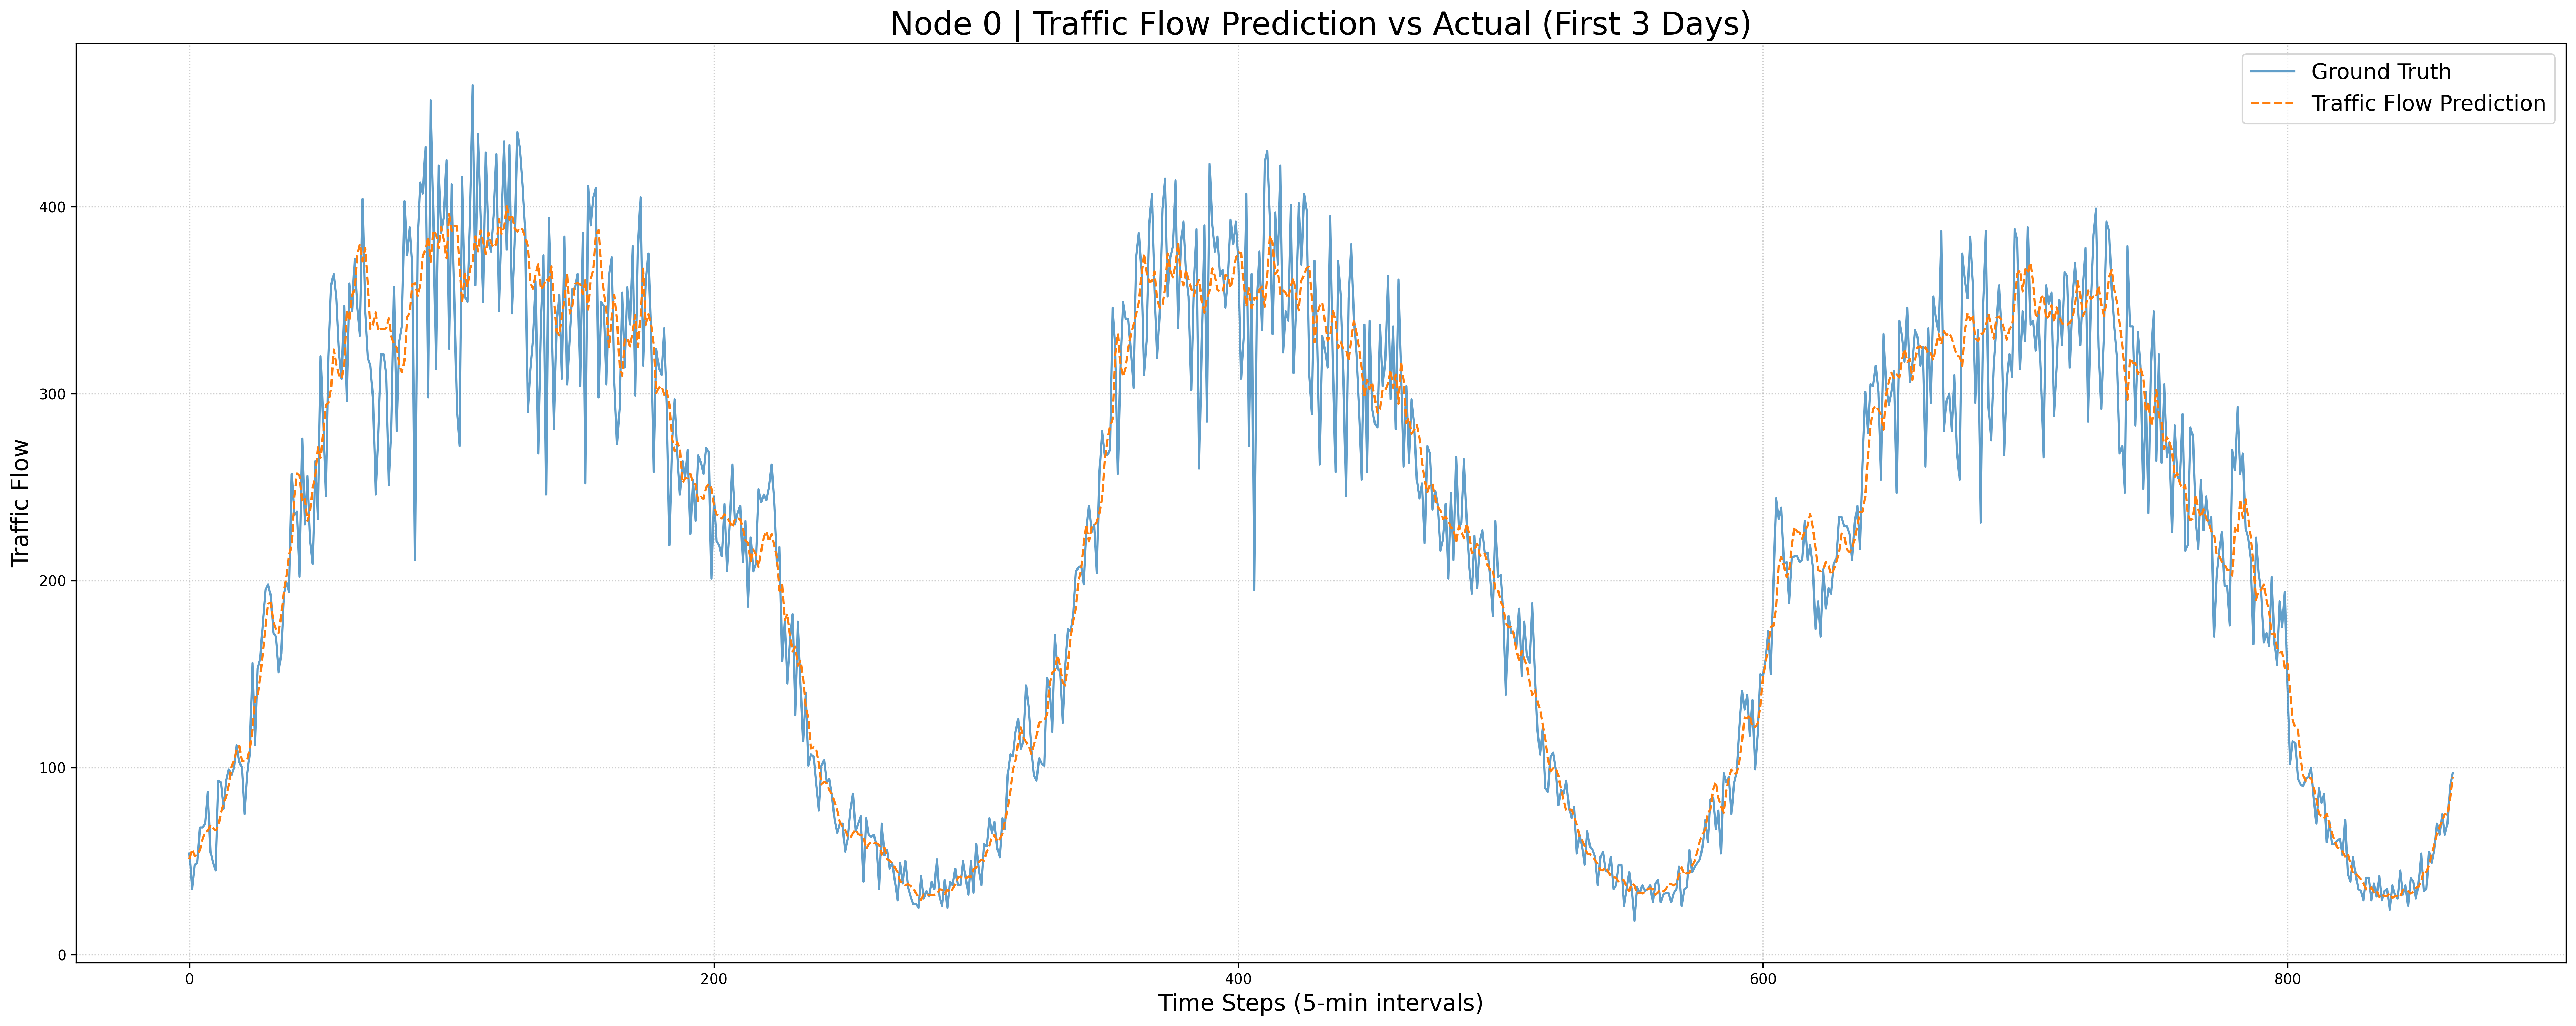
\includegraphics[width=0.85\textwidth]{figure/image5.png}
    \caption{PeMS08 测试集预测值与真实值对比}
    \label{fig:prediction-compare}
\end{figure}

\section{Agent指令解析与执行能力验证}

前两节验证了时空预测模型的预测精度，但系统最终的价值体现在智能体能否准确理解用户指令并正确调用工具。本节从指令理解、工具调度和端到端执行三个维度对智能体进行系统性评估。实验基于批量测试框架，在相同的本地部署环境中逐条读取测试用例，调用编译好的 LangGraph 工作流，记录每条用例的完整推理过程和最终输出结果。大模型使用本地 GPU 服务器上通过 vLLM 部署的 Qwen3.5-9B。底层工具链包括态势查询接口、历史趋势查询接口和 BIGCity 流量预测接口。

\subsection{指令理解与意图识别准确率评估}

评估从四个方面展开。第一是意图识别准确率，智能体能否根据用户指令正确选择三个工具之一，或在不需要工具时直接回复。第二是工具调度正确性，智能体能否正确提取实体 ID 和时间参数，特别是时间参数使用了中文口语、阿拉伯数字、斜杠分隔和点分隔等多种格式。第三是报告生成质量，智能体在收到工具返回的原始数据后能否组织出条理清晰的分析报告。第四是异常处理鲁棒性，遇到传感器 ID 越界、时间超出范围等情况时能否给出有意义的错误提示。

测试用例共 37 条，按照任务类型和难度分为七类：基础查询（8 条）、深度分析（11 条）、流量预测（8 条）、多工具协同（6 条）、无工具调用（1 条）、异常输入（2 条）和密集并行（1 条）。用例设计覆盖了全部三个工具类型，时间表述包括了中文书面语（七月一日）、带分隔符的数字（7.3、2016/7/2）和相对时间（昨天）等多种格式，任务复杂度从单工具单参数逐步递增到多工具多参数的复合任务。

意图识别是智能体决策链路的第一个关键环节。如果这一步出错，后续的所有工具调用都会偏离用户目标。表 \ref{tab:intent-accuracy} 统计了 37 条用例的意图识别结果。

\begin{table}[!htbp]
\centering
\caption{意图识别准确率统计}
\label{tab:intent-accuracy}
\begin{tabular}{p{3.5cm}p{1.5cm}p{1.5cm}p{1.5cm}p{1.8cm}}
\toprule
\textbf{任务类型} & \textbf{用例数} & \textbf{正确数} & \textbf{错误数} & \textbf{准确率} \\
\midrule
基础查询 & 8 & 8 & 0 & 100\% \\
深度分析 & 11 & 11 & 0 & 100\% \\
流量预测 & 8 & 8 & 0 & 100\% \\
多工具协同 & 6 & 6 & 0 & 100\% \\
无工具调用 & 1 & 1 & 0 & 100\% \\
异常输入 & 2 & 2 & 0 & 100\% \\
密集并行 & 1 & 1 & 0 & 100\% \\
\midrule
\textbf{合计} & \textbf{37} & \textbf{37} & \textbf{0} & \textbf{100\%} \\
\bottomrule
\end{tabular}
\end{table}

全部 37 条用例的意图识别均正确。对于工具调用类任务，智能体准确地选择了对应的工具类型。对于无工具调用类的第 34 条（"你好，请问你能帮我做什么呢"），智能体正确判断不需要调用工具，直接生成了文本回复，向用户介绍了实时查询、深度分析、流量预测和时间处理四大核心功能。这条用例验证了条件路由中 should\_continue 到 END 路径的有效性。

除了工具类型的选择，工具参数的提取同样关键。在 36 条需要工具调用的用例中，所有 entity\_id 和 time 参数的提取均正确。时间表述格式覆盖了五种常见自然语言习惯，表 \ref{tab:time-format} 给出了具体的覆盖情况。

\begin{table}[!htbp]
\centering
\caption{时间格式覆盖与解析结果}
\label{tab:time-format}
\begin{tabular}{p{4cm}p{4cm}p{2cm}p{2cm}}
\toprule
\textbf{时间格式} & \textbf{示例} & \textbf{出现次数} & \textbf{解析成功} \\
\midrule
中文书面语 & 2016 年七月一日上午十点 & 9 & 9 \\
数字+点分隔 & 2016.7.30 早上八点 & 5 & 5 \\
斜杠分隔 & 2016/7/2 18:00 & 3 & 3 \\
ISO-8601 风格 & 2016-07-08 晚上八点 & 4 & 4 \\
相对时间（昨天） & 昨天 14 点左右 & 3 & 3* \\
\bottomrule
\end{tabular}
\end{table}

从表中可以看出，智能体对五种时间格式的解析均未出现错误。智能体能够将"早高峰八点"映射为 08:00:00，将"傍晚六点"映射为 18:00:00，说明系统提示词中的时间基准设置为模型提供了足够的上下文锚点。第 7、8、19 条使用了"昨天"表述，智能体正确地将其解析为系统当前日期的前一天，但由于数据集仅覆盖 2016 年 7 至 8 月，查询返回空结果。这属于数据覆盖范围的问题而非时间解析错误，在接入实时数据流后这类查询将能正常工作。

在多工具协同用例中，参数提取的难度显著增大。以第 30 条为例，用户指令为"对比 20 号、21 号传感器在 2016.7.13 早上七点和八点的流量，再分析 22 号中午十二点的趋势，最后预测 23 号当天傍晚六点的车流"。智能体需要从一段自然语言中提取四个实体 ID、四个时间点和三个工具类型，并将它们正确配对。实际运行结果显示，智能体准确完成了这个三层嵌套的参数提取任务。

\subsection{典型交互场景与执行链路分析}

本节从七类用例中选取有代表性的样本，展示智能体的完整推理过程和执行链路。

基础查询场景以第 1 条用例"帮我查下 1 号传感器在 2016 年七月一日上午十点的流量"为例。智能体首先解析用户意图，识别出需要调用 simple\_query 工具，然后提取实体 ID 为 1、时间为 2016-07-01 10:00:00，生成工具调用指令。工具执行节点调用后端接口，返回流量 416 辆/小时、占有率 13.5\%、速度 61.0 km/h。智能体收到结果后将原始数据中的单位从 veh 转换为"辆"，生成格式清晰的分析报告。当查询涉及多个传感器时，智能体还能自动进行横向对比。第 4 条查询 24 号和 25 号探头的数据后，智能体不仅列出了各自的数值，还分析了两者的流量差异（60 vs 221 辆，相差近 4 倍），最后给出"两处路段均处于较为通畅的状态"的综合结论。

深度分析场景以第 9 条用例"能分析一下 2 号探头在 2016.7.1 下午五点半那会儿的交通情况吗"为例。智能体在一次推理中生成了两个工具调用：先调用 simple\_query 获取当前时刻的数据，再调用 deep\_analysis 拉取前后一段时间的连续历史序列。两条调用互不依赖，被工具执行节点并发执行。智能体将返回的结果整合为三个层次的分析报告：当前状态概览（流量 420 辆、占有率 7.7\%、车速 60.1 km/h）、历史趋势分析（识别出 16:45 到 17:05 期间两次流量高峰）和综合研判（"整体处于中等负荷状态，未出现拥堵"）。第 16 条用例进一步增加了拥堵程度判断，智能体给出了明确的定量标准："占有率 8.23\%，低于拥堵阈值（通常 >15\% 为拥堵），属于畅通水平"。

流量预测场景以第 20 条用例"预测一下 3 号传感器从 2016 年 7 月 2 日早上八点开始未来半小时的车流"为例。智能体调用 predict\_traffic 工具，该工具自动遍历全路网所有传感器节点拉取历史数据，组装时空特征矩阵后调用 BIGCity 推理引擎。智能体返回了 7 个时间步（每 5 分钟一个）的预测值，从 325 辆波动上升至 350 辆。报告不仅列出了预测数值表，还给出了趋势研判：08:05 出现短暂低谷（310 辆），随后从 08:20 起呈线性增长态势。第 21 条用例要求预测未来 1 小时，智能体返回了 12 个时间步的完整序列，并自动识别出 12:25 到 12:45 为"高位平台期"。

多工具协同场景以第 29 条用例为例，用户指令为"先帮我看看 16 号和 17 号传感器 2016 年 7 月 10 日上午 9 点的数据，再重点分析 16 号当天 18 点晚高峰"。智能体在第一阶段使用 simple\_query 获取了两个传感器在 09:00 的数据，发现 17 号流量（210 辆/小时）约为 16 号（94 辆/小时）的 2.2 倍。第二阶段使用 deep\_analysis 分析 16 号在当天 18:00 的状态，正确将"当天"解析为 2016-07-10。智能体从历史趋势中识别出 17:30 为流量峰值（146 辆/小时），随后回落至 18:00 的 131 辆/小时，综合评估为"未出现严重拥堵"。这条用例验证了智能体在多步推理中保持上下文一致性的能力。

异常处理场景中，第 35 条输入了超出范围的传感器 ID（200 号），智能体发起的 simple\_query 调用返回未找到数据的提示，智能体在报告中如实说明"未找到 200 号传感器的交通流量数据"，并给出了三种可能原因，全程未编造任何数据。第 36 条输入了超出数据集时间范围的预测请求，预测引擎返回"历史数据不足"的错误，智能体将其转化为用户可理解的"无法预测"提示。

密集并行场景中，第 37 条要求 3 个传感器乘以 3 个时间点共 9 次独立查询。智能体在一次推理中并行发起了全部查询，工具执行节点同时分发了所有请求。智能体将 9 组数据整理为按传感器分组的详细报告，并给出了跨传感器对比结论。

从全部用例的执行结果来看，智能体在意图识别、格式解析和工具调度方面表现稳定。所有成功的查询都返回了包含标题、数据表格、分析段落和结论的结构化报告，格式的一致性说明系统提示词对输出规范的约束是有效的。在异常处理方面，智能体对传感器不存在、时间超范围、历史数据不足等情况均做出了有意义的降级处理，未出现崩溃或幻觉。